\documentclass[pl]{minipw} % wszystkie ustawienia szablonu są w minipw.cls; if in English, change [pl] to [en]
\allowdisplaybreaks
\usepackage{indentfirst}
\setlength{\parindent}{5mm} % wcięcie akapitowe 5mm, zarządzenie Rektora

% ------------ Ustawienia autora pracy ---------------
\title{Agent system for HVAC management in office building} % nazwa pracy
\titleaux{Agentowy system zarządzania urządzeniami HVAC w budynku biurowym}

\type{magisters} % licencjat = licencjac, inżynier = inżyniers
\discipline{Informatyka} % kierunek
\specjal{Metody sztucznej inteligencji}

\author{Jan Grzybowski}
\setboolean{lady}{false} % kobiety wpisują true, mężczyźni - false
\album{245491}

\supervisor{dr~hab. Marcin Paprzycki}
\konsultacje{dr~hab Maria Ghanza} % jeśli nie ma, trzeba zakomentować też w minipw.cls
\date{2017}
\klucze{Wieloagentowy, HVAC, aktorzy}
\keywords{Multi-agent, HVAC, actors}
% ----------------------------------------------------

\usepackage{color}
\usepackage[dvipsnames]{xcolor}
\usepackage{listings}

\lstset{ % General setup for the package
	language=[Sharp]C,
	%Font
  basicstyle=\ttfamily,
  %Line numbering
  numbers=left, 
  numberstyle=\ttfamily,
	%Frame & border
  frame=tb,
  %Whitespaces
	tabsize=2, columns=fixed,
	showtabs=false,
	keepspaces,
  showstringspaces=false,
	%Coloring
  commentstyle=\color{green},
	keywordstyle=\color{teal},
  stringstyle=\color{red}
}

\begin{document}
\sloppy
  
\setcounter{page}{1}

% 2. Streszczenia
% Streszczenie ma zawierać tytuł pracy i słowa kluczowe
\begin{streszczenie}  
???Lorem ipsum dolor sit amet, consetetur sadipscing elitr, sed diam nonumyeirmod tempor invidunt ut labore et dolore magna aliquyam erat, sed diamvoluptua. At vero eos et accusam et justo duo dolores et ea rebum. Stet clita kasd gubergren, no sea takimata sanctus est Lorem ipsum dolor sit amet.???\\
\end{streszczenie}


\begin{abstract}
???Lorem ipsum dolor sit amet, consetetur sadipscing elitr, sed diam nonumyeirmod tempor invidunt ut labore et dolore magna aliquyam erat, sed diamvoluptua. At vero eos et accusam et justo duo dolores et ea rebum. Stet clita kasd gubergren, no sea takimata sanctus est Lorem ipsum dolor sit amet.

Lorem ipsum dolor sit amet, consetetur sadipscing elitr, sed diam nonumyeirmod tempor invidunt ut labore et dolore magna aliquyam erat, sed diamvoluptua. At vero eos et accusam et justo duo dolores et ea rebum. Stet clita kasd gubergren, no sea takimata sanctus est Lorem ipsum dolor sit amet.???\\
\end{abstract}
    

% 3. Oświadczenie o autorstwie pracy - w innym pliku
\makestatement

% 4. Spis treści
\cleardoublepage
\tableofcontents


% 5. Treść
\cleardoublepage
\pagestyle{fancy}

\chapter{Wprowadzenie}
Jendym z zastosowań teleinformatyki w dzisiejszych czasach jest monitorowanie i automatyzacja procesów zachodzących w budynkach mieszkalnych i biurowych. 
W większości nowoczesnych budynków biurowych zamontowane są liczne urządzenia zapewniające komfortowe warunki pracy osób przebywających w biurach takie jak np. klimatyzatory czy nawilżacze powietrza. Te jak i inne urządzenia HVAC (Heating, Ventilation, Air Conditioning czyli ogrzewanie, wentylacja i klimatyzacja) mają moc liczoną w kilowatach.

Opłata za energię elektryczną potrzebną do funkcjonowania sieci takich urządzeń, jest częścią kosztu mediów (prądu, wody, ogrzewania, odprowadzania ścieków), które średnio stanowią ponad jedną trzecią miesięcznych kosztów utrzymania budynku \cite{bib:raportKoszty}.

Założeniem systemu tworzonego na potrzeby tej pracy jest obniżenie kosztów związanych z działaniem klimatyzacji z zachowaniem komfortu użytkowników budynku. 
System będzie miał do dyspozycji informacje zbierane z sensorów (małych czujników odczytujących wartości różnych parametrów) rozmieszczonych w każdym biurze oraz dane o wykorzystaniu pomieszczeń. \seefigure{generalContextDiagram}

\begin{figure}[bth]
    \centering
    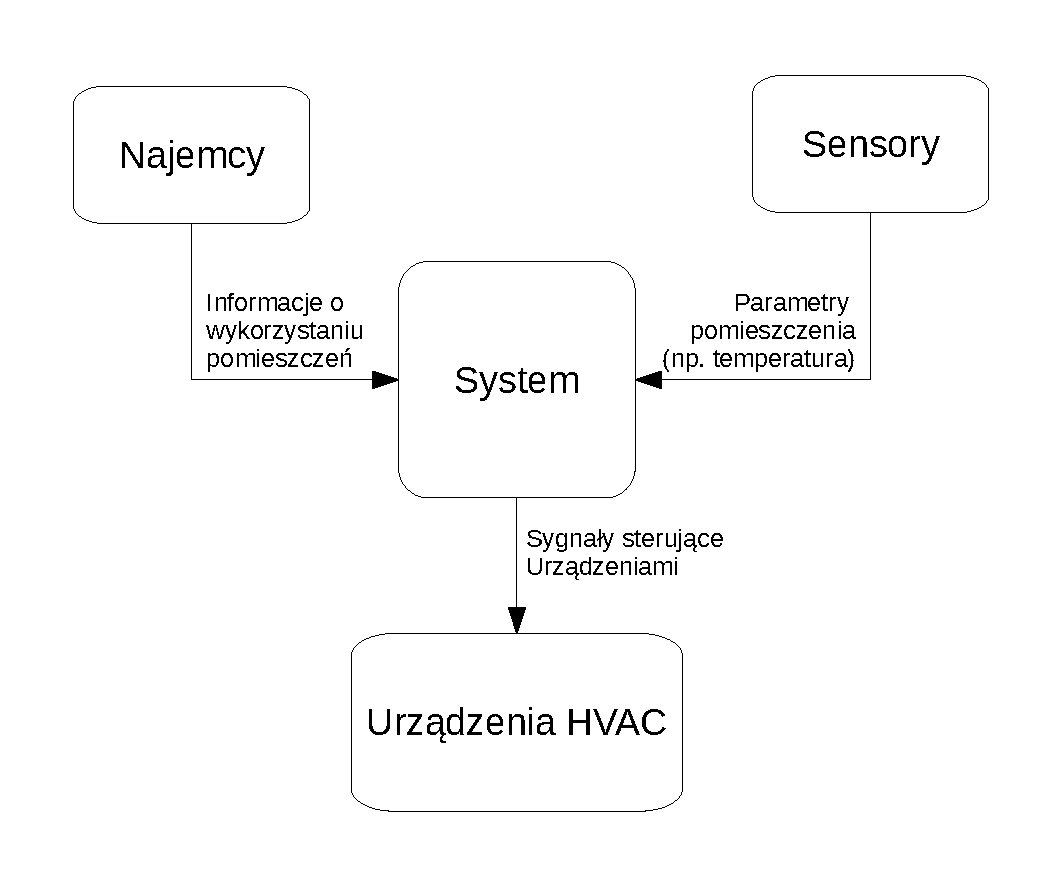
\includegraphics[width=0.7\textwidth]{./diagrams/GeneralContextDiagram.pdf}
    \caption{Kontekst systemu}
    \label{fig:generalContextDiagram}    
\end{figure}
 

Kalendarze firmowe są głównym źródłem informacji, w których pomieszczeniach i w jakich godzinach, odbywają się spotkania. Można wyobrazić sobie inne źródła, jak np. lokalizacja pracowników przypisanych do pomieszczenia. 
Jednak implementowany system będzie skupiał się głównie na wydarzeniach firmowych, jako że są mniej dynamiczne i można za ich pomocą zamodelować również np. spóźniającego się pracownika przesuwając godzinę spotkania.

System będzie sterował urządzeniami HVAC poprzez aktuatory (urządenia pozwalające komputerowi wpływać na stan świata rzeczywistego), które mogłyby składać się z mikrokomputerów z portami podczerwieni lub komunikacją radiową (Bluetooth czy WiFi.)
Aktuatory wyręczałyby użytkowników w prawidłowym ustawianiu urządzeń.
Przy ręcznym ustawianiu komfortowej temperatury przez człowieka zwykle odbywa się to na początku spotkania, gdy uczestnicy uznają, że warunki w pomieszczeniu nie odpowiadają ich wymaganiom. 
Aby jak najszybciej pozbyć się tego uczucia, włączają najmocniejszy, lecz nie koniecznie najbardziej oszczędny, tryb w klimatyzatorach.

Oszczędność z zastosowania systemu będzie przychodzić z uruchomienia klimatyzatorów przed spotkaniem w najbardziej ekonomicznym wariancie tak, aby uczestnicy mieli komfortowe warunki od początku aż do końca spotkania. 

Do wyliczenia, ile czasu wcześniej należy uruchomić urządzenia, potrzebne są matematyczne modele zjawisk, takich jak wymiana ciepła. 
Tworzeniem precyzyjnych modeli takich zajwisk zajmują się inne dziedziny techniki - ogrzewnictwo oraz chłodnictwo. 
Jako, że opracowanie dokładnych modeli jest poza zakresem tej pracy system będzie korzystał z modelu uproszczonego. 

\chapter{Analiza biznesowa}
\section{Omówienie zagadnienia}
W większości budynków biurowych zamontowane są klimatyzatory, które zapewniają komfortowe warunki pracy osób przebywających w biurach. 
Ilość prądu potrzebnego do funkcjonowania sieci takich urządzeń jest sporą częścią miesięcznych kosztów dla właściciela budynku.

Przy ręcznym ustawianiu komfortowej temperatury przez człowieka zwykle odbywa się to na początku spotkania gdy uczestnicy uznają, że warunki w pomieszczeniu nie odpowiadają ich wymaganiom. Aby jak najszybciej pozbyć się tego uczucia włączają najmocniejszy, lecz nie koniecznie najbardziej oszczędny, tryb w klimatyzatorach.

Założeniem implementowanego w tej pracy systemu jest ustalanie temperatury komfortu przed spotkaniem i uruchomienie klimatyzatorów przed spotkaniem w najbardziej ekonomicznym wariancie, tak aby uczestnicy mieli komfortowe warunki od początku spotkania i utrzymanie ich przez całe spotkanie. 

Głównym źródłem informacji w których pomieszczeniach i w jakich godzinach odbywają się spotkania są kalendarze firmowe. Można wyobrazić sobie inne źródła takie jak lokalizacja pracowników przypisanych do pomieszczenia, jednak implementowany system będzie skupiał się głównie na wydarzeniach firmowych, jako że są mniej dynamiczne i można za ich pomocą zamodelować również np. spóźniającego się pracownika przesuwając godzinę spotkania.

Przewidzieć ile czasu wcześniej należy uruchomić urządzenia i w jakim trybie można za pomocą matematycznych modeli. Przygotowanie dokładniejszych modeli nie mieści się w zakresie pracy, przyjęto zatem prosty model opierający się o moc i wydajność urządzeń. 

\section{Analiza wymagań systemu}
Przy założeniu ewentualnej późniejszej rozbudowy systemu lub przeniesienia go na inny język programowania system musiał spełniać następujące wymagania:

\subsection*{Możliwość dodania nowych parametrów pomieszczenia}
Dodanie nowych parametrów takich jak wilgotność czy nasłonecznienie pozwalałoby udoskonalić model temperatur i zbliżyć go do rzeczywistego modelu fizycznego.

Jednocześnie dodanie takich parametrów jak poziom tlenu w pomieszczeniu dawałby możliwość sprawdzenia czy osobom w pomieszczeniu nie jest zbyt duszno oraz przewietrzenia pomieszczenia za pomocą dostępnych urządzeń.

Oczywiście każde dodanie takiego parametru wiązałoby się z nowym typem sensora i w niektórych przypadkach aktuatora o ile badane zajwisko zmianiałoby się na tyle wolno, że moglibyśmy na nie oddziałowywać.

\subsubsection*{Parametryzacja i podmiana modeli}
Możliwość parametryzacji model pozwoliłaby dostrajać modele i poprawić precyzję działania i sugesti systemu.

Podmiana modeli umożliwiłaby aktualizację parametrów modelu lub podmianę na inaczej skonstruowany model (np. przewidujący temperatury z innych parametrów pomieszczenia) bez wyłączania systemu . 

\subsection*{Możliwość podpięcia różnych źródeł danych}
W różnych firmach używa się różnych systemów do ustalania terminów spotkań czy rezerwacji sal np. Microsoft Exchange Server czy IBM Domino. 

System powinien pozwalać na dopisanie adaptera zajmującego się przekazywaniem wydarzeń do systemu HVAC i uniezależnianiem go od źródła danych.

\subsection*{Możliwość zbadania stanu systemu}
Dla celach diagnostycznych oraz aby dostroić modele potrzebne są dane o stanie urządzeń oraz dane z samego systemu HVAC. Musi zatem istnieć sposób, aby w łatwy sposób połączyć się z systemem HVAC i zerbać informacje o jego stanie.

\section{Analiza wymagań aplikacji symulatora}

\subsection{Schemat budynku}
\subsection{Scenariusze}


\chapter{Architektura rozwiązania}
\chapter{Testy}

\chapter{Wnioski i podsumowanie}
\section{Podsumowanie}
\section{Wnioski}
Systemy agentowe, a w szczególności systemy aktorów są wygodnym narzędziem do zarządzania siecią urządzeń. 
W perspektywie coraz większej popularności internetu rzeczy (IoT - Internet of Things) można spodziewać się też co raz częstszego wykorzystania tych rozwiązań w zastosowaniach już nie tylko przemysłowych, jak automatyzacja fabryk, ale i konsumenckich jak automatyka biur lub domów.  

Wykorzystanie tradycyjnych technik znanych z programowania obiektowego, takich jak zdarzenia, w systemie aktorów nie jest możliwe ze względu na zasady przydzielania wątków poszczególnym aktorom. Również 
korzystanie z kontenerów do wstrzykiwania zależności wewnątrz aktorów może prowadzić do dzielenia stanu przez aktorów, co jest sprzeczne z założeniami Akka.net i samego modelu aktorów.

\section{Propozycje dalszego rozwoju systemu}
\subsection*{Dodanie nowych parametrów pomieszczeń}
Powszechnie dostępne sensory temperatury często posiadają również czujnik wilgotności, która wpływa na to, jak szybko nagrzewa się powietrze. Monitorowanie wilgotności pozwalałoby na dokładniejsze wyliczenia zmian temperatury. Zbyt wysoka wilgotność mogłaby być czynnikiem wyzwalającym wietrzenie, aby osobom w pomieszczeniu nie był zbyt duszno.

\subsection*{Udoskonalenie strategii uruchamiania urządzeń}
Zaproponowana strategia uruchamiania urządzeń zakłada uruchamianie wszystkich urządzeń w pomieszczeniu w tym samym trybie na ten sam okres czasu. Być może opracowanie strategii gdzie pewne urządzenia pełnią rolę pomocniczą przez część czasu przygotowywania pomieszczenia dawałoby dodatkowe oszczędności.

\subsection*{Opracowanie nowych źródeł danych}
Przy omawianiu źródeł danych wspomniane zostały alternatywy do kalendarzy firmowych. Przykładowo lokalizacja użytkowników pozwoli zaoszczędzić energię elektryczną, gdy pracownik firmy tkwi przez godzinę w korku i spóźnia się do swojego biura. 

Lokalizacja wewnątrz samego budynku też wydaje się dobrym źródłem informacji o wykorzystaniu pomieszczeń, lecz może okazać się zbyt dynamiczna, aby móc ją wykorzystać w planowaniu.

\subsection*{Douczanie modelu na podstawie danych z systemu}
Pomieszczenia w biurowcach różnią się rozmiarami, kształtem oraz rozmieszczeniem urządzeń HVAC. Powoduje to, że każde z nich ogrzewa się inaczej. Jeżeli dodać do aktora kontrolera moduł poprawiający model temperatury dla danego pomieszczenia, możemy jeszcze bardziej zoptymalizować koszty energii elektrycznej.

\subsection*{Wykorzystanie osobistych preferencji użytkowników}
Jedną z trudniejszych rzeczy dla użytkowników korzystających z proponowanego systemu może być określenie z wyprzedzeniem jaka temperatura będzie dla nich komfortowa.
Zbudowanie modułu w którym byłaby przechowywana informacja o preferowanych temperaturach pozwoliłoby na sugerowanie temperatury podczas spotkania. 

% 6. Bibliografia
% Bibliografia leksykograficznie wg nazwisk autorów
\begin{thebibliography}{20}%jak ktoś ma więcej książek, to niech wpisze większą liczbę

% \bibitem[numerek]{referencja} Autor, \emph{Tytuł}, Wydawnictwo, rok, strony
% cytowanie: \cite{referencja1, referencja 2,...}
\bibitem[1]{bib:AkkaVsOrleans}Dr R. Kuhn, \emph{Orleans and Akka Actors: A Comparison} [dostęp: 07 XII 2017], https://github.com/akka/akka-meta/blob/master/ComparisonWithOrleans.md

% \bibitem[2]{Ktos} A. Aaaaa, \emph{Tytuł}, Wydawnictwo, rok, strona-strona.
% \bibitem[3]{Innyktos} J. Bobkowski, S. Dobkowski, \emph{Blebleble}, Magazyn nr, rok, strony.
% \bibitem[4]{B} C. Brink, \emph{Power structures}, Algebra Universalis 30(2), 1993, 177-216.
% \bibitem[0]{H} F. Burris, H. P. Sankappanavar, \emph{A Course of Universal Algebra}, Springer-Verlag, New York, 1981.

\end{thebibliography}

% 7. Wykaz symboli i skrótów - jeśli nie ma, zakomentować
% \chapter*{Wykaz symboli i skrótów}

% \begin{tabular}{cl}
% nzw. & nadzwyczajny \\
% * & operator gwiazdka \\
% $\widetilde{}$ & tylda
% \end{tabular}

% 8. Spis rysunków - jeśli nie ma, zakomentować (ale być może po prostu się nie zrobi)
% \listoffigures

% 9. Spis tabel - jak wyżej
% \renewcommand{\listtablename}{Spis tabel}
% \listoftables

% 10. Spis załączników - jak nie ma załączników, to zakomentować lub usunąć
% \chapter*{Spis załączników}
% \begin{enumerate}
% \item[1.] Załącznik 1
% \item[2.] Załącznik 2
% \end{enumerate}

% 11. Załączniki
% \newpage
% \pagestyle{empty}
% Załącznik 1, załącznik 2 -- mają się znajdować na końcu pracy (to jest notka przypominająca)


\end{document}
